%!TEX root = Constructive Alignment for Introductory Programming.tex

\chapter{Approaches to Constructive Alignment} % (fold)
\label{cha:background}

\graphicspath{{Figures/Background/}}

\cite{DeRaadt:2005} approach to learning  had the strongest correlation to success as compared to other cognitive and demographic measures.

\section{Constructive Alignment} % (fold)
\label{sec:constructive_alignment}

Constructive alignment, as proposed by Biggs~\cite{Biggs:1996c}, is an amalgamation of constructive learning theory and aligned instruction design. It aims to elicit deep learning approaches from all students. Biggs' model is student focused, with clear and intentional alignment of assessment, teaching and learning activities, and unit objectives. The focus on the central role of the learner in building meaning is derived from constructivist learning theories, whilst the alignment of assessment, teaching, and learning activities, has its foundation in instructional design literature. 

\fref{fig:constructive_alignment} illustrates the constructive alignment model presented in~\cite{Houghton:2004}, which consists of the following blocks:

\begin{itemize}
	\item \emph{Intended learning outcomes} clearly define required learning in terms of ``performances of understanding''.
	\item \emph{Performance objectives} emerge from the desired outcomes, and can be ranked to become the assessment criteria.
	\item \emph{Teaching and learning activities} are designed to place students in situations likely to elicit the required learning.
	\item Students provide \emph{evidence of their learning}, that is assessed against the criteria to determine grade outcomes.
\end{itemize}

% \begin{figure}[t!]
% 	\centering
% 	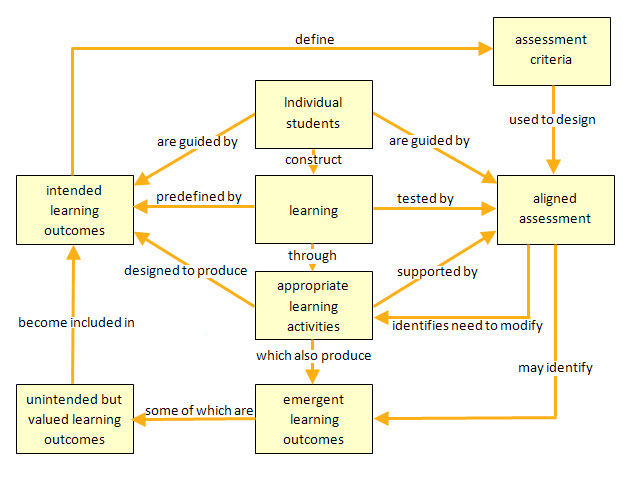
\includegraphics[width=\columnwidth]{Houghton_constructive_alignment_1}
% 	\caption{Constructive alignment model presented by Houghton in~\cite{Houghton:2004}}
% 	\label{fig:constructive_alignment}
% \end{figure}

\subsection{Constructivism} % (fold)
\label{sub:constructivism}

In designing teaching and learning contexts, educators use some form of theory of teaching and learning to guide their decision making.

theory of teaching and learning

espoused theory \cite{Argyris:1976}

\emph{objectivist}

\emph{constructivism} and \emph{phenomenography}


\cite{Duffy:1996} 




\cite{Montessori:1946}

Constructivism is a theory of knowledge that focuses on the active role of the learner in constructing their own understanding. Dating back to \citet{Piaget:1950} constructivism exists in several forms: cognitive, individual, postmodern, radical and social constructivism \cite{Phillips:1995,Steffe:1995}. Each of these forms of constructivism has various implications for teaching and learning.









In his original paper on constructive alignment \citet{Biggs:1996c} adopted constructivism as a framework to help guide decision making in all facets of teaching and learning. Constructivism was chosen over phenomenography 

practical concerns


For this work we are interested in adapting \emph{constructive learning theories}

 taking practical aspects from constructivism in general and focusing on what the student does, as suggested by .


In proposing constructive alignment, 

Disconnect between theory in use and espoused theory: \cite{Phillips:2005}


Engage with and expand experience \cite{Dewey:1960} exploration, thinking and reflection

% subsection constructivism (end)

\subsection{Aligned Curriculum} % (fold)
\label{sub:aligned_curriculum}

% subsection aligned_curriculum (end)


% section constructive_alignment (end)

\clearpage
\section{Reported Applications of Constructive Alignment} % (fold)
\label{sec:reported_applications_of_constructive_alignment}

In this section we outline a literature review that examined the applications of constructive alignment in Higher Education. This review aimed to help identify how constructive alignment can be applied to introductory programming, and any gaps in the current research literature. 

\subsection{Review Method} % (fold)
\label{sub:review_method}

\citet{Petticrew:2008} define a structure literature review as a process of systematically analysing all available studies in order to answer specific research questions.This work followed the structured literature review process of \citet{Kitchenham:2004}, and aimed to identify all available studies on how Constructive Alignment has been applied in Higher Education.

\fref{fig:struct_review_proc} shows the three phases in the structured literature review carried out in this work. The first phase identified appropriate search and filter criteria to be used in locating associated literature. In Phase 2, the search criteria is used to identify potentially relevant articles from the indicated sources. The articles identified are then filtered using the filter criteria to identify the relevant articles to pass on to Phase 3, where relevant data is collected from the articles are the analysis performed.

\begin{figure}[tbph]
	\centering
	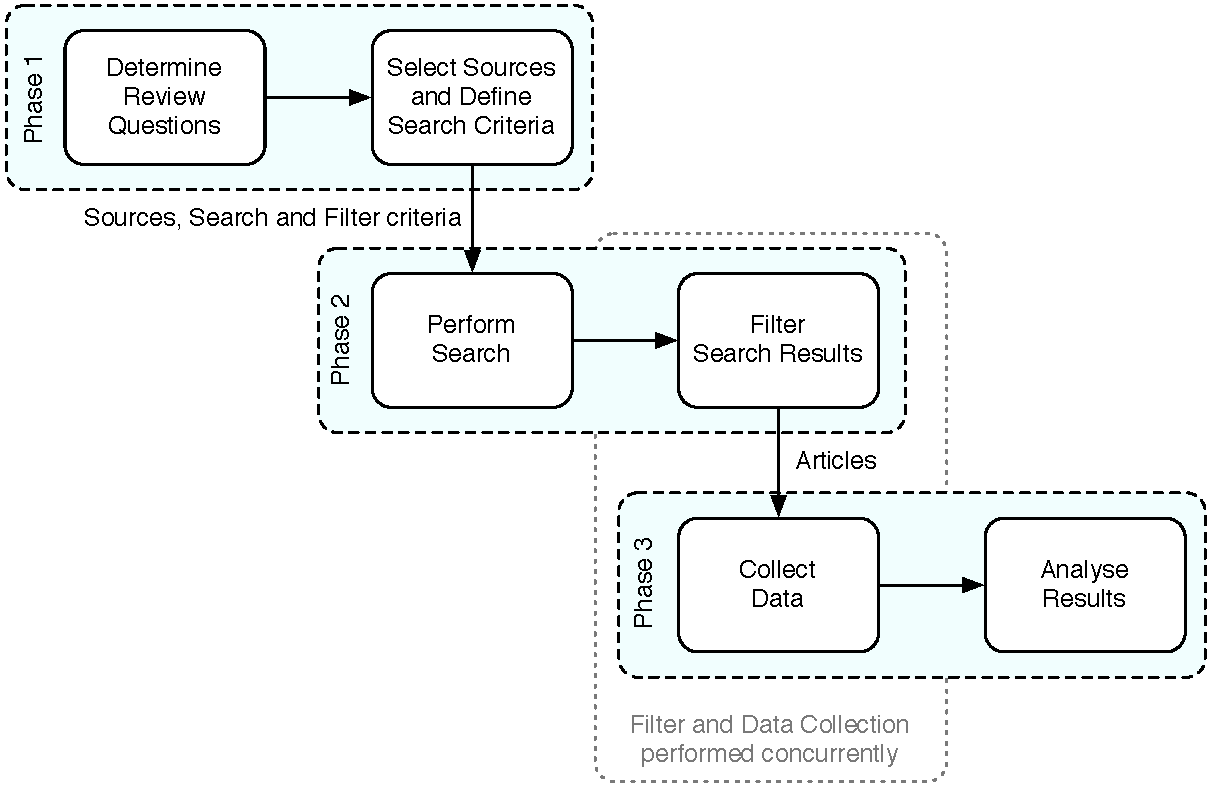
\includegraphics[width=\textwidth]{SystematicReview}
	\caption{Processes in the Structured Literature Review process carried out in this work}
	\label{fig:struct_review_proc}
\end{figure}



\subsubsection{Approach to Phase 1} % (fold)
\label{sub:review_questions}

This review focused on the application of constructive alignment, and the effectiveness of the teaching and learning environment created. \citet{Petticrew:2008} suggest that the formulation of research questions for a systematic review should consider five aspects: Population, Intervention, Comparison, Outcome and Context (PICOC). Addressing these five aspects enable effective search and filter criteria, that will then be used to identify related work for the review to analyse.

\tref{tbl:picoc} lists the five PICOC aspects related to this review. The Population consists of the specific target group that the study will examine. In this study, the population included students and academics in the context of Higher Education. This work aimed to review interventions where academics had applied the principles of Constructive Alignment, and any comparisons they had with their existing approaches to teaching and learning. In terms of outcomes, we were interested in examining any positive or negative impacts these changes had on either the staff or the students.

\begin{table}[h]
	\centering
	\caption{Focus for database search using PICOC}
	\label{tbl:picoc}

    \begin{tabular}{|l|p{8cm}|}
    \hline
    \textbf{Population} & Students and Academics in Higher Education\\ \hline
    \textbf{Intervention} & Applications of Constructive Alignment in the design of teaching and learning activities and assessment. \\ \hline
    \textbf{Comparison} & Existing approaches \\ \hline
    \textbf{Outcomes} & Positive and negative impacts on student learning, as well as impacts on teaching staff. \\ \hline
    \textbf{Context} & Application of Constructive Alignment to the design and delivery of teaching and learning material in a Higher Education setting. \\ \hline
    \end{tabular}
\end{table}


This structured literature review aimed to answer the following questions:

\begin{enumerate}[noitemsep,nolistsep]
	\item What evidence is there of studies on the application of constructive alignment to teaching and learning in higher education?
	\item How has the effectiveness of constructive alignment been measured in these studies, and how effective has constructive alignment been in the higher education setting?
	\item What teaching and learning activities are used in conjuncture with constructive alignment?
	\item What forms of assessment have been used with constructive alignment?
	\item In what ways have applications of constructive alignment addressed the two main elements of constructive alignment: constructivism and aligned curriculum?
\end{enumerate}

\citet{Petticrew:2008} described the need for the search criteria to result in high number of relevant articles, while excluding irrelevant ones. These are referred to as the search criteria sensitivity and specificity. A search with high sensitivity returns a high number of relevant articles, one with high specificity a low proportion of irrelevant articles. While an ideal search criteria would be both highly sensitive and highly specific, there generally tends to be a trade-off between the two. 

\citet{Kitchenham:2004} provides a number of recommendations on how to define appropriate search criteria, including the use of Boolean AND and OR conditions as well as searching for synonyms. Using this approach results in a search with higher specificity, and can result in a low number of articles being identified, see \citet{Salleh:2011} for example. Therefore, for this work it was decided to start with a highly \emph{sensitive} search criteria, and search for articles that match the term ``Constructive Alignment''. If this resulted in a unacceptably large number of results then more specific criteria could be added.

Filter

% subsection research_questions (end)

\subsubsection{Identification of Relevant Literature} % (fold)
\label{ssub:identification_of_relevant_literature}






% subsubsection identification_of_relevant_literature (end)

\subsubsection{Data Collection and Analysis} % (fold)
\label{ssub:data_collection_and_analysis}

% subsubsection data_collection_and_analysis (end)


% subsection review_method (end)

\subsection{Results} % (fold)
\label{sub:review_results}

The search involved the use of seventeen online databases, as listed in \tref{tbl:review_source}.

\begin{savenotes}
\begin{table}[ht]
	\centering
	\caption{Data sources and the number of articles located for the search term ``Constructive Alignment''.}
	\label{tbl:review_source}
	\footnotesize
    \begin{tabular}{l|l|c}
    \textbf{Source} & \textbf{URL} & \textbf{Count} \\ \hline
    A+ Education & \url{http://search.informit.com.au/search} & 44 \\
    Academic Search Complete & \scriptsize \url{http://ebscohost.com/academic/academic-search-complete} & 32 \\
    ACM Digital Library & \url{http://dl.acm.org} & 21 \\
    CiteSeer\footnote{With CiteSeer the search was performed on article abstracts containing the text ``Constructive Alignment''.}  & \url{http://citeseerx.ist.psu.edu} & 20 \\
    EdResearch Online & \url{http://opac.acer.edu.au:8080/edresearch} & 6 \\
    Educational Research Abstracts & \url{http://www.tandfonline.com} & 26 \\
    Education Research Complete & \scriptsize \url{http://ebscohost.com/academic/education-research-complete} & 48 \\
    eJournals & \url{http://ejournals.ebsco.com} & 42 \\
    ERIC & \url{http://www.eric.ed.gov} & 31 \\
    Google Scholar\footnote{The search in Google scholar returned more than three thousand results, this was then limited to articles that included ``Constructive Alignment'' in their title.} & \url{http://scholar.google.com} & 104 \\
    IEEE Xplore & \url{http://ieeexplore.ieee.org} & 16 \\
    Libra & \url{http://academic.research.microsoft.com} & 87\\
	PsycINFO & \url{http://ebscohost.com/academic/psycinfo} & 16 \\
	Scopus & \url{http://www.scopus.com/} & 79 \\
	Springer Link & \url{http://link.springer.com} & 125 \\
	VOCED & \url{http://www.voced.edu.au} & 28 \\
	Web of Knowledge & \url{http://wokinfo.com} & 52 \\ \hline
	Total Unique & & 335 \\
    \end{tabular}
\end{table}
\end{savenotes}










\begin{table}[htbp]
	\centering
	\caption{Counts of number of papers excluded by reason}
	\label{tbl:exclude_reason}
	\footnotesize
    \begin{tabular}{ll}
    \textbf{Reason} & \textbf{Count} \\ \hline
    Excluded on First Pass & 77 \\
    No Mention of Constructive Alignment & 33 \\
    Excluded on Second Pass & 96 \\
    Not a study of a Teaching \& Learning Context & 43 \\
    Not an application of Constructive Alignment & 23 \\
    Duplicates & 10 \\ \hline
    Applications of Constructive Alignment & 53 \\
    \end{tabular}
\end{table}


% subsection results (end)

% section reported_applications_of_constructive_alignment (end)


\section{Constructive Alignment in Introductory Programming} % (fold)
\label{sec:constructive_alignment_in_introductory_programming}

% section constructive_alignment_in_introductory_programming (end)

\section{Closing Comments} % (fold)
\label{sec:closing_comments}

% section closing_comments (end)

% chapter background (end)